\chapter{Walkthrough of a \Penrose Trio for Euler Diagram}
\label{app:penrose-trio-walkthrough}

In this section, we walk through a trio of \Substance, \Style, and \Domain programs for making Euler diagrams of sets in \Penrose. We demonstrate how to define sets, specify subset relationships, and use constraints to adjust the layout of Euler diagrams. Note that the syntax in this appendix reflects the latest of \texttt{@penrose/core@4.0.0-alpha.3}, which includes some changes since the writing of \cref{chp:penrose}.

The goal of this walkthrough is to create Euler diagrams of sets represented as circles with text labels, as shown in \cref{fig:sets-euler}.

\begin{figure}[h!]
    \centering
    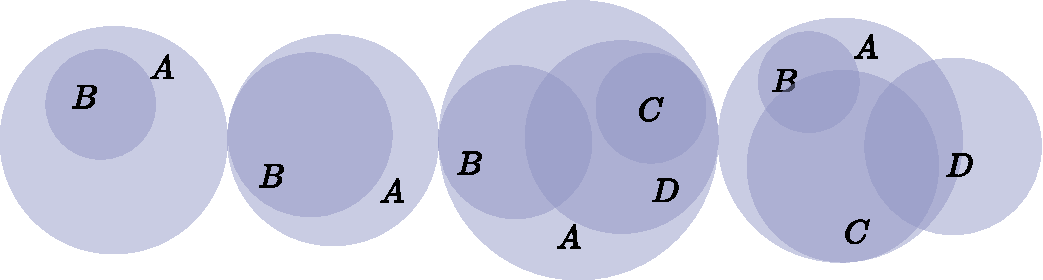
\includegraphics[width=.9\linewidth]{assets/appendix/sets-euler.pdf}
    \caption{Example Euler diagrams made in \Penrose}
    \label{fig:sets-euler}
\end{figure}

\section{\Domain program for sets}

\begin{center}
\begin{mdframed}[style=DSLCode]
\begin{lstlisting}[language=Elem,escapechar=@]
type Set@\label{lin:set}@
predicate Subset(Set s1, Set s2)@\label{lin:subset}@
\end{lstlisting}
\end{mdframed}
\end{center}

We first define the language of sets and set relations in the \Domain language. \Domain lets the user declare possible concepts in diagrams for a particular domain. Here we define sets as a type of object (Line~\ref{lin:set}), and subset relations as a predicate that takes two sets as arguments (Line~\ref{lin:subset}).

\section{Declaring Sets and Subset Relations in \Substance}
\label{sec:euler-substance}

Once \Domain is defined, we can define the sets and their relationships in the declarative format of \Substance. The program below defines four sets: \(A\), \(B\), \(C\), and \(D\) (Line~\ref{lin:sets-decl}). We state that $B, C, D \subset A$ and $C \subset D$~(Line~\ref{lin:subsets-decl-1}--\ref{lin:subsets-decl-2}), the \Substance program and one corresponding diagram shown in \cref{fig:euler-sub-example}.

\begin{figure}[h]
    \centering
    \begin{minipage}{.25\linewidth}
    \begin{mdframed}[style=SUBCode]
    \begin{lstlisting}[language=Sub-SET-new,escapechar=@]
Set A, B, C, D@\label{lin:sets-decl}@
Subset(B, A)@\label{lin:subsets-decl-1}@
Subset(C, A)
Subset(D, A)
Subset(C, D)@\label{lin:subsets-decl-2}@
AutoLabel All@\label{lin:label-decl}@\end{lstlisting}
    \end{mdframed}
    \end{minipage}\hspace{2em}
    \begin{minipage}{.3\linewidth}
    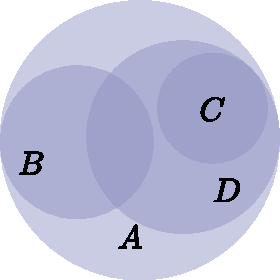
\includegraphics[width=\linewidth]{assets/appendix/Sets as Euler Diagram 1.pdf}
    \end{minipage}
    \caption{An example \Substance program in the set theory domain illustrated with the Euler diagram \Style.}
    \label{fig:euler-sub-example}
\end{figure}

Line~\ref{lin:label-decl} generates label strings from the \Substance identifiers (\eg the string values such as \texttt{"A"} and \texttt{"B"}) automatically. The user has an option to specify labels that are different from the identifiers by an explicit label declaration statement such as \inlineSUB{\texttt{\keyword{Label} A \$\textbackslash{}Gamma\$}}. We will discuss how these labels are used for styling in the next section.


\section{Styling Euler Diagrams using \Style}

With the objects and relations declared, we need to specify their visual representations. In \Penrose, \Style is the language that maps from abstract objects to visual icons and relations. For every \Style program, we need to define the canvas size. In this case, we specify a canvas width and height of \texttt{200} pixels. Note that \Penrose generates vector images, so the size is only relative to the sizes of shapes on the canvas. 

\begin{center}
\begin{mdframed}[style=STYCode]
\begin{lstlisting}[language=Sty-Sets-new,escapechar=@]
canvas {
  width = 200
  height = 200
}
\end{lstlisting}
\end{mdframed}
\end{center}

The visual appearance of the sets is determined by the \Style program. The selector on Line~\ref{lin:selector} selects all \texttt{Set} in the \Substance program (\cref{sec:Selectors}). Lines~\ref{lin:circle}--\ref{lin:layer} declare shapes and visual relations for each \texttt{Set}. 

\begin{center}
\begin{mdframed}[style=STYCode]
\begin{lstlisting}[language=Sty-Sets-new,escapechar=@]
forall Set X {@\label{lin:selector}@
  X.shape = Circle { fillColor: #8C91C277 }@\label{lin:circle}@
  X.text  = Equation { string: X.label }@\label{lin:equation}@
  ensure contains(X.shape, X.text)@\label{lin:contains}@
  X.text above X.shape@\label{lin:layer}@
}
\end{lstlisting}
\end{mdframed}
\end{center}

Line~\ref{lin:circle} represents each set as a \keyword{Circle} with a specific fill color, specified using a hexadecimal RGBA value of a translucent purple. Note that the size and position of the \keyword{Circle} is left unspecified, the concrete  values of which will be automatically determined by \Penrose at runtime. 

Similar to Line~\ref{lin:circle}, Line~\ref{lin:equation} declares an \keyword{Equation} shape for each \keyword{Set}. \keyword{Equation} is a built-in shape type that renders as a \LaTeX{} label in math mode. The string content of the \keyword{Equation} is determined by the \texttt{string} property. Here we use \texttt{X.label} to refer to the label text specified in \Substance (\cref{sec:euler-substance}). The \texttt{label} field is reserved for label strings specified in \Substance. Since the \Substance uses \keyword{AutoLabel All}, each set will get an \keyword{Equation} shape with a string content of its \Substance identifier, $A,B,C$ and so forth.

Now that we have both the \keyword{Circle} and \keyword{Equation} for each \keyword{Set}, we need to position them properly so the \keyword{Equation} is always in the \keyword{Circle} for clear labeling. Line~\ref{lin:contains} specifies a constraint that ensures that the label always appears inside its corresponding circle. \texttt{contains} is one of the constraint functions in the \Penrose library\footnote{\url{https://penrose.cs.cmu.edu/docs/ref/style/functions\#constraint-contains}}, which ``Require that a shape contains another shape, based on the type of the shape, and with an optional padding between the sizes of the shapes.''

Finally, the layering statement on Line~\ref{lin:layer} ensures that the \keyword{Equation} is always on top of the \keyword{Circle} for good label visibility. Internally, \Penrose takes these partial orderings (\eg \texttt{A.text} is \keyword{above} \texttt{A.shape}) and produce a global orderings in the rendered SVG that respects all layering statements in \Style. In the case of cycles in the partial orderings, \Style produces a cycle-free layer list via an algorithm that attempts to break cycles while preserving partial orderings as much as possible. \cref{fig:euler-partial-1} show an example diagram generated by \Penrose after writing down this \Style block.

\begin{figure}[h!]
    \centering
    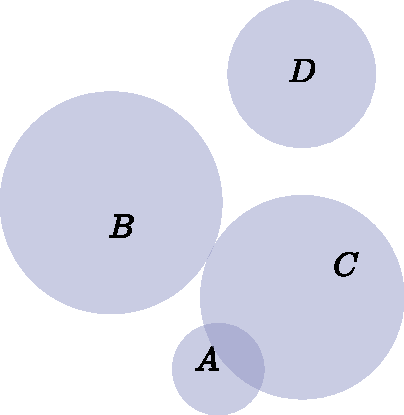
\includegraphics[width=.4\linewidth]{assets/appendix/after-set-block.pdf}
    \caption{\Penrose-generated diagram after the \texttt{forall Set X} Euler diagram \Style block.}
    \label{fig:euler-partial-1}
\end{figure}

The subset relationships between the sets are handled by another block of \Style code. Note the \keyword{where} clause in the selector on Line~\ref{lin:where} will match on all \keyword{Set}s with \keyword{Subset} predicates declared between them.

\begin{center}
\begin{mdframed}[style=STYCode]
\begin{lstlisting}[language=Sty-Sets-new,escapechar=@]
forall Set X, Y where Subset(X, Y) {@\label{lin:where}@
  ensure contains(Y.shape, X.shape)@\label{lin:subset-contains}@
  ensure disjoint(Y.text, X.shape)@\label{lin:subset-disjoint}@
  X.shape above Y.shape@\label{lin:subset-layer}@
}
\end{lstlisting}
\end{mdframed}
\end{center}

Line~\ref{lin:subset-contains} ensures that whenever a \keyword{Set} \(X\) is a \keyword{Subset} of another \keyword{Set} \(Y\), the \keyword{Circle} representing \(X\) is always inside the \keyword{Circle} representing \(Y\). The `disjoint` constraint on Line~\ref{lin:subset-disjoint} prevents the label of the larger set \(Y\) from overlapping the circle of the subset \(X\) for better label clarity. Line~\ref{lin:subset-layer} makes sure the subset \keyword{Circle} (and by extension the \keyword{Equation} too) is always on top of the superset \keyword{Circle}.

\section{Layout Optimization and Rendering}

\begin{figure}[h!]
    \centering
    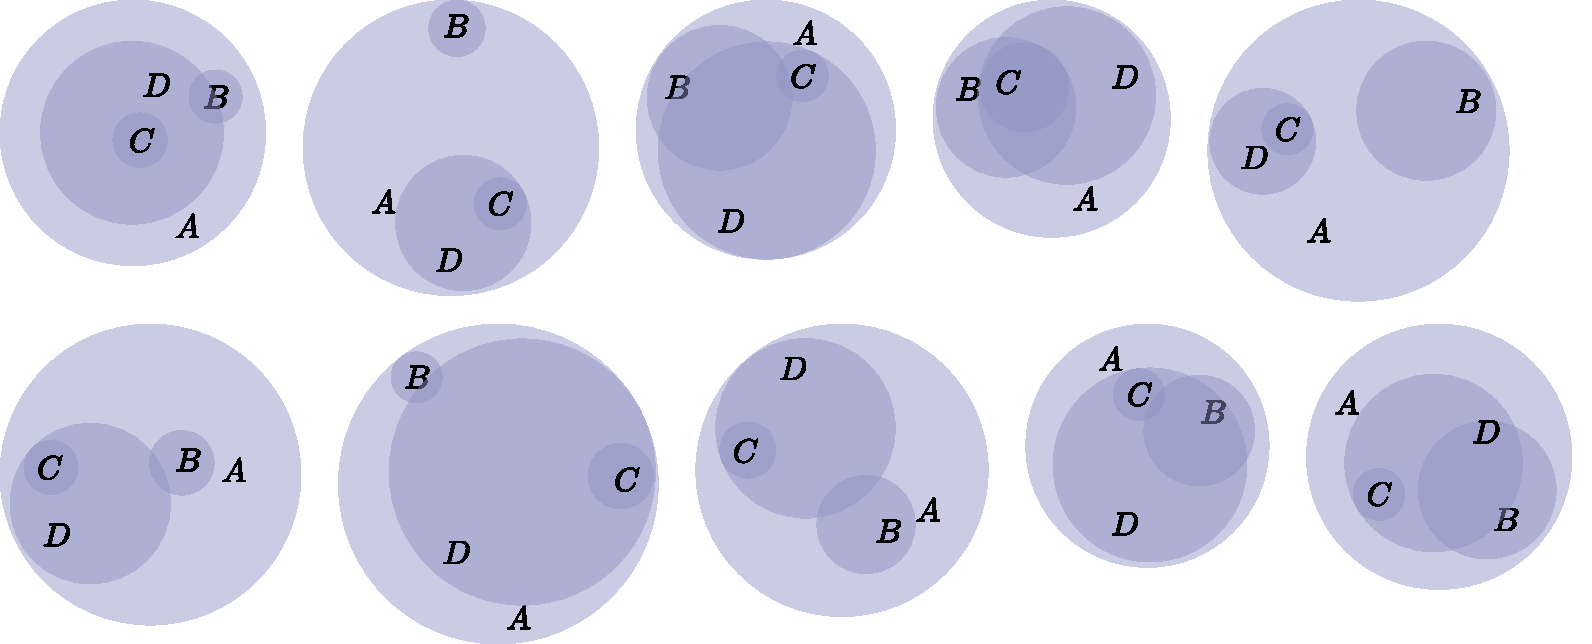
\includegraphics[width=\linewidth]{assets/appendix/sets-variations.pdf}
    \caption{Variations of the same \Substance program for sets rendered with different intializations using the ``resample'' mechanism in \Penrose.}
    \label{fig:sets-variations}
\end{figure}

Once we have defined our sets, subset relations, and visual constraints, we can execute the Penrose program to generate the diagram. Each time the diagram is generated, \Penrose ensures that all constraints are satisfied, and we can even modify the \Substance program (\eg adding or removing sets or relations) while maintaining the visual consistency of the diagram.

By using the ``resample'' button in Penrose, we can regenerate the diagram with different initializations while keeping the subset relations intact. \cref{fig:sets-variations} shows 10 samples generated by \Penrose for the same \Substance program.
